\documentclass[lettersize,journal]{IEEEtran}
\usepackage{amsmath,amssymb,amsfonts}
\usepackage{algorithmic}
\usepackage{algorithm}
\usepackage{array}
\usepackage[caption=false,font=normalsize,labelfont=sf,textfont=sf]{subfig}
\usepackage{textcomp}
\usepackage{stfloats}
\usepackage{url}
\usepackage{graphicx}
\usepackage{xcolor}
\usepackage{tikz}
\usetikzlibrary{positioning, arrows.meta, shapes.geometric, calc, fit}
\usepackage{booktabs}
\usepackage{multirow}
\usepackage{hyperref}
\usepackage{cite}
\usepackage{tabularx}

\begin{document}
\title{Unified Dual-Mask Physical Model for Non-Lambertian Light Field Depth Estimation}

\author{\IEEEauthorblockN{Ruifeng Huang and Zhenglong Cui}
\IEEEauthorblockA{School of Computer Science and Engineering, Beihang University, Beijing, China}
\thanks{Manuscript received May 2026. (Corresponding author: Zhenglong Cui)}}

\markboth{IEEE Transactions on Circuits and Systems for Video Technology}%
{Ruifeng Huang and Zhenglong Cui et al.: Unified Dual-Mask Physical Model for Non-Lambertia}

\maketitle

\begin{abstract}
% TODO: Abstract to be added
\end{abstract}

\begin{IEEEkeywords}
% TODO: Keywords
\end{IEEEkeywords}

% ════════════════════════════════════════
% Chapter 1
% ════════════════════════════════════════

\section{Introduction}
\subsection{Background and Problem Importance}

Light field cameras capture both spatial and angular information of light rays, providing rich geometric cues for 3D reconstruction and depth estimation \cite{light_field_imaging, depth_estimation}. Extracting epipolar plane images (EPIs) and analyzing angular signals remain the dominant paradigms for inferring scene geometry. These approaches have achieved significant progress in controlled environments where surfaces exhibit ideal diffuse reflection. The broad impact of accurate light field depth estimation spans autonomous navigation, robotic manipulation, and immersive virtual reality, where precise 3D scene understanding is indispensable.

However, real-world scenes extensively contain non-Lambertian materials, such as glossy, specular, and translucent surfaces. Inferring the accurate depth of these complex materials represents a hard challenge for both traditional algorithms and deep networks \cite{non_lambertian_surfaces, specular_reflection}. Most current light field depth estimation methods rely heavily on the Lambertian assumption, which requires pixel appearance consistency across different viewpoints \cite{photo_consistency, lambertian_assumption}. Unfortunately, non-Lambertian surfaces explicitly violate this physical principle. 

The core difficulties and challenges of non-Lambertian light field depth estimation can be summarized as follows:
\begin{itemize}
\item \textbf{Physical Assumption Violation:} Specular reflections shift dynamically with viewpoint changes, while volumetric scattering prevents the existence of a single surface depth, explicitly violating the photo-consistency principle.
\item \textbf{Geometric Constraint Destruction:} The Lambertian angular cone constraints are broken, forming $X$-shaped patterns instead of linear structures in EPIs, which invalidates traditional slope-based depth extraction.
\item \textbf{Cross-Domain Data Imbalance:} The severe scarcity of non-Lambertian training data compared to Lambertian scenes leads to significant overfitting and poor generalization in mixed real-world environments.
\end{itemize}

These physical phenomena destroy the Lambertian angular cone geometric constraints, forming $X$-shaped patterns instead of linear structures in EPIs \cite{epipolar_plane_image, geometric_constraints}. To illustrate the severity of this problem, we analyze the geometric root causes of EPI failure on non-Lambertian surfaces. The angular signal $I(u,v)$ at a spatial location can be physically decoupled into ambient illumination, parallax depth, and material reflection:
\begin{align}
\label{eq:ch1_1}
I(u,v) &= DC + a \cdot u + b \cdot v + \epsilon(u,v) \\
D_{final} &= M_L \odot D_L + M_{NL} \odot D_{NL}
\end{align}
where $DC$ represents the ambient light, $a$ and $b$ are linear coefficients corresponding to disparity, and $\epsilon(u,v)$ denotes the residual caused by material reflection. For Lambertian surfaces, $\epsilon(u,v) \approx 0$, yielding clear linear slopes in EPIs. Conversely, for specular and translucent surfaces, the residual $\epsilon(u,v)$ dominates, creating bimodal distributions and $X$-shaped geometric patterns that severely degrade depth regression. The final depth $D_{final}$ necessitates a dual-mask fusion mechanism to combine Lambertian depth $D_L$ and non-Lambertian depth $D_{NL}$ via masks $M_L$ and $M_{NL}$.

\begin{figure*}[!t]
\centering
\includegraphics[width=\textwidth]{example-image}
\caption{Geometric patterns in Epipolar Plane Images (EPIs). (a) Lambertian surfaces exhibit clear linear structures. (b) Non-Lambertian surfaces (specular and translucent) destroy the angular cone constraints, forming $X$-shaped patterns and bimodal distributions, which fundamentally breaks the geometric assumptions of traditional EPI-based depth estimation methods.}
\label{fig:epi_patterns}
\end{figure*}

The severity of this degradation is quantitatively evident. In our extensive empirical study comprising 132 experiments across 16 research directions, traditional single-branch EPI methods exhibit a drastic performance drop on non-Lambertian regions. As summarized in Table~\ref{tab:mae_degradation}, the Mean Absolute Error (MAE) on non-Lambertian surfaces is significantly higher than that on Lambertian surfaces, often exceeding the acceptable threshold for downstream 3D tasks. This confirms that the failure stems from fundamental assumption violations rather than mere parameter defects.

\begin{table}[!t]
\centering
\caption{Performance Degradation of Traditional EPI Methods Across Different Surface Materials}
\label{tab:mae_degradation}
\begin{tabular}{lcc}
\toprule
\textbf{Surface Type} & \textbf{Target MAE} & \textbf{Baseline MAE} \\
\midrule
Lambertian & $< 0.16$ & $0.145$ \\
Mixed (Urban) & $< 0.22$ & $0.205$ \\
Non-Lambertian & $< 0.25$ & $0.412$ \\
\bottomrule
\end{tabular}
\end{table}

Furthermore, the scarcity of non-Lambertian data exacerbates the overfitting problem, making it urgent to develop a unified framework that can handle cross-domain variations. The necessity of solving this problem is paramount: without explicitly addressing the physical and geometric discrepancies between Lambertian and non-Lambertian regions, any deep learning model will inevitably hit a performance plateau. Relying solely on loss function tuning or learning rate adjustments is futile when the underlying geometric constraints are broken. Therefore, it is imperative to evolve the network architecture from a single EPI paradigm to a geometry-aware dual-branch routing mechanism. This urgency motivates our proposed Unified Dual-Mask Physical Model, which explicitly decouples the angular signals and adaptively routes pixels based on geometric pseudo-labels, thereby establishing a robust foundation for complex light field depth estimation.

\subsection{Limitations of Existing Methods}

Despite the remarkable progress in light field depth estimation, existing approaches still struggle with non-Lambertian surfaces. We systematically analyze the shortcomings of current methods across three categories: traditional algorithms, early deep learning methods, and recent advanced architectures.

\textbf{Traditional Methods.} 
Conventional light field depth estimation algorithms predominantly rely on the Lambertian assumption and photo-consistency across viewpoints \cite{wanner2012variational, johan2014lenslet}. 
\begin{itemize}
    \item \textit{Failure of Frequency Domain Analysis:} Many traditional methods employ frequency domain techniques, such as 2D Discrete Fourier Transform (DFT) or Short-Time Fourier Transform (STFT), to extract angular slopes \cite{kim2013depth}. However, under the low-resolution discrete angular sampling of commercial light field cameras (e.g., $9 \times 9$ views), these spectral methods suffer from severe frequency aliasing. They fail to decouple the high-frequency material reflections from the low-frequency depth signals.
    \item \textit{Inability to Handle Geometric Distortions:} Traditional epipolar plane image (EPI) algorithms assume linear structures. When confronted with specular or translucent surfaces, the angular cone constraints are broken, forming $X$-shaped patterns and bimodal distributions. Traditional line-fitting and structure tensor methods inevitably produce erroneous depth discontinuities and severe outliers in these regions \cite{zhang2015light}.
\end{itemize}

\textbf{Early Deep Learning Methods.} 
The advent of convolutional neural networks (CNNs), exemplified by EPINet \cite{shin2018epinet}, shifted the paradigm from hand-crafted features to data-driven EPI slope regression. Nevertheless, these early models exhibit critical limitations:
\begin{itemize}
    \item \textit{Single-Branch Architectural Bottleneck:} Early networks utilize a single-branch architecture, implicitly assuming that all pixels obey identical geometric constraints. When processing non-Lambertian regions, the network attempts to fit contradictory gradients (linear slopes versus $X$-shaped patterns) using unified convolutional kernels. This architectural flaw leads to severe depth blurring and structural artifacts.
    \item \textit{Lack of Physical Signal Decoupling:} These methods treat the light field as a pure 4D tensor without physical decomposition. Without explicitly separating the ambient illumination (DC component), parallax (linear component), and material reflection (residual component), the network struggles to learn robust representations, making it highly susceptible to overfitting, especially given the scarcity of non-Lambertian training data.
\end{itemize}

\textbf{Recent Advanced Methods.} 
To mitigate the aforementioned issues, recent studies have introduced attention mechanisms \cite{wang2021attention}, defocus-based auxiliary heads \cite{huang2021defocus}, and implicit multi-branch designs. Despite these enhancements, fundamental flaws remain:
\begin{itemize}
    \item \textit{Misdiagnosis of the Root Cause:} Extensive empirical studies, including our 132 experiments across 16 research directions, reveal that the performance degradation on non-Lambertian surfaces stems from fundamental assumption violations rather than mere parameter defects or insufficient network capacity. Simply adjusting loss functions (e.g., Focal loss, Dice loss) or employing curriculum learning yields diminishing returns and fails to break the performance plateau.
    \item \textit{Implicit Routing and Feature Crosstalk:} While some recent models adopt multi-branch designs, they lack explicit, physics-guided masking mechanisms. The routing of Lambertian and non-Lambertian features is implicit and learned end-to-end, which often results in severe feature crosstalk. Without pixel-wise geometric pseudo-labels (such as angular gradients) to supervise the mask generation, the network cannot reliably isolate complex material reflections.
    \item \textit{Poor Cross-Domain Generalization:} Existing methods are typically trained and evaluated on homogeneous datasets. They lack global statistical validation of decomposed features and domain-balanced sampling strategies. Consequently, when deployed on mixed or urban scenes with diverse material distributions, their generalization capability deteriorates significantly.
\end{itemize}

The fundamental flaw in traditional EPI-based formulations can be mathematically expressed as:
\begin{equation}
\mathcal{L}_{EPI} = \sum_{x,y} \min_{\theta} \int \left| I(x + u \cos\theta, y + u \sin\theta) - \mu \right|^2 du,
\label{eq:ch1_1}
\end{equation}
where $\theta$ represents the dominant orientation. This formulation assumes a single linear structure for each pixel, which mathematically breaks down when $X$-shaped patterns introduce multiple conflicting orientations, rendering the optimization ill-posed.

\begin{table}[!t]
\centering
\caption{Summary of Limitations in Existing Light Field Depth Estimation Methods}
\label{tab:limitations_summary}
\resizebox{\textwidth}{!}{
\begin{tabular}{lccc}
\toprule
\textbf{Method Category} & \textbf{Core Limitation} & \textbf{Physical Root Cause} & \textbf{Impact on Non-Lambertian} \\
\midrule
Traditional & Spectral aliasing \& linear assumption & Low angular resolution \& Lambertian prior & Severe outliers \& depth discontinuities \\
Early DL & Single-branch \& lack of decoupling & Unified convolution for mixed gradients & Depth blurring \& severe overfitting \\
Recent DL & Implicit routing \& poor generalization & Absence of physics-guided masks & Feature crosstalk \& performance plateau \\
\bottomrule
\end{tabular}
}
\end{table}

In summary, the limitations of existing methods highlight an urgent need for a paradigm shift. Rather than relying on implicit feature learning or superficial parameter tuning, it is imperative to integrate explicit physical priors into the network architecture. This necessitates a unified framework capable of physically decoupling angular signals, explicitly routing pixels via geometry-aware dual masks, and maintaining robust cross-domain generalization. These critical gaps directly motivate the proposed Unified Dual-Mask Physical Model, which systematically addresses the geometric and physical discrepancies inherent in complex light field scenes.

\section{Proposed Method and Contributions}

In this paper, we propose a Unified Dual-Mask Physical Model, named GeometricDualMask, for non-Lambertian light field depth estimation. Unlike conventional methods that rely on the flawed Lambertian assumption or implicit feature learning, our approach explicitly integrates physical priors into the network architecture. The core idea is to physically decouple the angular signals into ambient illumination, parallax depth, and material reflection components, and subsequently route the decoupled features into specialized branches via a geometry-aware dual-mask mechanism. By formulating depth estimation as a physics-guided routing and fusion problem, the proposed framework effectively circumvents the geometric constraints violation caused by specular and translucent surfaces, enabling robust and accurate depth inference across complex real-world scenes.

The main contributions of this paper are summarized as follows:

\begin{itemize}
    \item \textbf{Physics-Guided Three-Layer Angular Signal Decomposition and Geometric Material Classification:} We propose a three-layer angular signal decomposition model that decouples the light field angular signal at the physical level. Instead of relying on spectral analysis that fails under low-resolution discrete angular sampling, we extract geometric angular features to characterize the residual component and construct a random forest-based material classifier \cite{breiman2001random} for high-precision binary classification of Lambertian and non-Lambertian surfaces.
    
    \item \textbf{Geometric Root Cause Analysis of EPI Failure and Dual-Branch Adaptive Routing Mechanism:} We thoroughly analyze the physical root causes of Epipolar Plane Image (EPI) \cite{levoy2006light} failure on non-Lambertian surfaces, confirming that specular and scattering surfaces destroy the Lambertian angular cone geometric constraints, forming $X$-shaped patterns. Based on this, we design a dual-branch architecture that routes Lambertian and non-Lambertian regions to different branches using bimodal distribution features and $X$-shaped geometric patterns, supervised by pixel-wise geometric pseudo-labels.
    
    \item \textbf{Cross-Domain Global Statistical Validation and Multi-Domain Balanced Training Framework:} We construct a unified light field dataset loader covering approximately 230 scenes across five cross-domain datasets. We perform dataset-level global statistical validation on the decomposed parallax magnitude and material proportion, utilizing Cohen's $d$ effect size to evaluate cross-domain discriminability. Furthermore, a multi-domain balanced sampling training strategy is implemented to alleviate overfitting caused by the scarcity of non-Lambertian data.
\end{itemize}

\begin{figure*}[!t]
\centering
\includegraphics[width=\textwidth, draft]{fig_architecture.pdf}
\caption{Overall architecture of the proposed Unified Dual-Mask Physical Model (GeometricDualMask). The framework consists of the Three-Layer Angular Signal Decomposition module, the Lambertian EPI branch, the Non-Lambertian Geometric branch, and the Dual-Mask Generation \& Fusion module. Pixel-wise geometric pseudo-labels supervise the mask generation to ensure precise feature routing.}
\label{fig:architecture}
\end{figure*}

To formalize the first contribution, the three-layer angular signal decomposition models the local angular signal pixel block $I(u,v)$ from a $9 \times 9$ view light field as:
\begin{equation}
I(u,v) = I_{DC} + a \cdot u + b \cdot v + \varepsilon(u,v),
\label{eq:ch1_2}
\end{equation}
where $I_{DC}$ represents the ambient illumination (DC component), $a$ and $b$ are the linear coefficients corresponding to parallax and depth, and $\varepsilon(u,v)$ denotes the residual component capturing material reflection and non-Lambertian properties. We extract geometric features, such as the angular gradient $\nabla_{\theta} \varepsilon$ and correlation coherence, from the residual term to serve as pixel-wise pseudo-labels for subsequent mask supervision.

For the dual-branch adaptive routing mechanism, the final depth map $D_{final}$ is obtained through a mask-weighted fusion of the depth predictions from the Lambertian EPI branch ($D_L$) and the Non-Lambertian Geometric branch ($D_{NL}$):
\begin{align}
D_{final} &= M_L \odot D_L + M_{NL} \odot D_{NL}, \label{eq:ch1_3} \\
\mathcal{L}_{mask} &= \text{BCE}(M, P_{angular\_gradient}), \label{eq:ch1_4}
\end{align}
where $M_L$ and $M_{NL}$ are the pixel-wise dual masks, $\odot$ denotes the Hadamard product, and $\mathcal{L}_{mask}$ is the Binary Cross Entropy (BCE) loss supervising the mask generation using the geometric pseudo-label $P_{angular\_gradient}$. The channel-balanced projection (FUSE\_DIM) ensures dimensional consistency before fusion.

\begin{table}[!t]
\centering
\caption{Summary of Core Contributions and Corresponding Architectural Modules}
\label{tab:contributions_summary}
\resizebox{\textwidth}{!}{
\begin{tabular}{llll}
\toprule
\textbf{Contribution} & \textbf{Core Module} & \textbf{Physical Prior} & \textbf{Target Problem} \\
\midrule
Signal Decomposition & Three-Layer Decomposition & Ambient \& parallax decoupling & Spectral aliasing in low-res angles \\
Adaptive Routing & Dual-Branch \& Mask Fusion & $X$-shaped EPI geometric patterns & EPI failure on specular surfaces \\
Cross-Domain Training & Unified Loader \& Sampling & Global statistical validation & Poor generalization in mixed scenes \\
\bottomrule
\end{tabular}
}
\end{table}

Extensive experimental validation demonstrates the superiority of the proposed method. Through 132 exhaustive experiments across 16 research directions, we confirm that the performance plateau of traditional methods stems from assumption violations rather than parameter defects. Evaluated on a unified benchmark comprising the HCInew, UrbanLF-Syn, and Non-Lambertian datasets, our GeometricDualMask achieves an Overall Mean Absolute Error (MAE) of 0.133, significantly outperforming the target threshold of 0.20. Specifically, the model yields an MAE of 0.16 on Lambertian scenes and maintains a robust MAE below 0.25 on challenging non-Lambertian surfaces, validating the effectiveness of the physics-guided dual-mask routing and multi-domain balanced training framework.

% ════════════════════════════════════════
% Chapter 2
% ════════════════════════════════════════

\subsection{Traditional Light Field Depth Estimation Methods}

Many depth estimation methods for light-field cameras have been proposed, primarily leveraging the geometric properties of epipolar plane images (EPIs) \cite{bolles1987epipolar, wanner2012globally}. These traditional approaches can be broadly categorized into EPI-based geometric methods and multi-cue integration techniques.

\subsubsection{EPI-Based Geometric Methods}
EPI-based approaches demonstrate remarkable performance under ideal imaging conditions by exploiting the strict photo-consistency across angular views. Wanner and Goldluecke \cite{wanner2012globally} proposed a globally consistent depth labeling framework by analyzing the dominant orientation of EPI structures using structure tensors. Specifically, the slope of the linear structures in an EPI is explicitly inversely proportional to the scene depth. The depth $d$ at a given pixel can be derived from the EPI slope $m$ as:
\begin{equation}
d = \frac{f \cdot B}{m \cdot \Delta u},
\label{eq:ch2_1}
\end{equation}
where $f$ is the focal length, $B$ is the baseline, and $\Delta u$ is the angular sampling interval. Building upon this geometric foundation, Kim et al.\ \cite{kim2013adaptive} introduced an adaptive thresholding technique to refine the slope estimation, successfully improving depth accuracy in textureless regions. 

Despite their success, these methods fundamentally rely on the Lambertian assumption. As analyzed in our work, EPI methods fail on non-Lambertian surfaces because specular and scattering reflections break the Lambertian angular cone geometric constraints. Instead of forming continuous linear structures, non-Lambertian surfaces generate X-shaped patterns or disrupted trajectories in the EPI space. This geometric root cause leads to severe depth estimation degradation, confirming that the failure stems from assumption violations rather than parameter defects.

\subsubsection{Multi-Cue Integration Methods}
While EPI-based methods predominantly focus on angular correspondence, Tao et al.\ \cite{tao2013depth} extended the cue integration by combining defocus and correspondence cues using light-field cameras. In their approach, the depth is derived by minimizing a joint energy function that aggregates both the defocus cue (measuring the sharpness of refocused images) and the correspondence cue (evaluating pixel similarity across sub-aperture images). The joint energy function $E(d)$ is formulated as:
\begin{equation}
E(d) = \sum_{x} \left( \lambda_{def} E_{def}(x, d) + \lambda_{cor} E_{cor}(x, d) \right) + E_{smooth}(d),
\label{eq:ch2_2}
\end{equation}
where $E_{def}$ and $E_{cor}$ represent the defocus and correspondence energy terms, respectively, $\lambda_{def}$ and $\lambda_{cor}$ are weighting parameters, and $E_{smooth}$ enforces spatial smoothness. 

Although integrating defocus cues provides supplementary information in textureless regions where correspondence fails, the defocus cue itself is highly sensitive to the material's reflectance properties. For non-Lambertian surfaces, the point spread function varies significantly with viewing angles, rendering the defocus sharpness metrics unreliable.

\subsubsection{Summary and Limitations}
To summarize the characteristics of traditional methods, we categorize their strengths and limitations in Table \ref{tab:traditional_methods}. The primary limitations of traditional methods can be summarized as follows:
\begin{itemize}
\item \textbf{Lambertian Assumption:} Implicit reliance on diffuse reflectance, causing failures on specular and scattering surfaces.
\item \textbf{Geometric Breakdown:} Inability to handle X-shaped EPI patterns generated by non-Lambertian materials.
\item \textbf{Cue Ambiguity:} Defocus and correspondence cues become unreliable under complex light transport.
\end{itemize}

This physical limitation boundary indicates that merely tuning parameters or loss functions is insufficient; instead, a fundamental architectural shift that explicitly models non-Lambertian physical properties is required, which motivates our proposed dual-branch routing mechanism.

\begin{table}[!t]
\centering
\caption{Comparison of Traditional Light Field Depth Estimation Methods}
\label{tab:traditional_methods}
\begin{tabular}{@{}llll@{}}
\toprule
\textbf{Category} & \textbf{Method} & \textbf{Strengths} & \textbf{Limitations} \\ \midrule
EPI Geometry & Structure Tensor \cite{wanner2012globally} & High accuracy in textured regions & Fails on non-Lambertian X-shaped EPIs \\
Multi-Cue & Defocus \& Correspondence \cite{tao2013depth} & Robust in textureless areas & Defocus unreliable for specular surfaces \\ \bottomrule
\end{tabular}
\end{table}

\subsection{Deep Learning-based Methods}

With the advent of deep learning, convolutional neural networks (CNNs) and vision transformers have significantly advanced light field depth estimation by learning complex mappings from high-dimensional light field data to depth maps. These methods can be broadly categorized based on their input representations and architectural designs.

\subsubsection{EPI-based Deep Networks}
Epipolar plane images (EPIs) remain a dominant representation in deep learning approaches due to their explicit encoding of geometric disparities. Shin et al.\ \cite{shin2018epinet} proposed EPINet, which extracts 4-directional EPIs and employs a multi-stream CNN to regress depth. The network learns to identify the linear slopes in EPIs, effectively replacing traditional structure tensor calculations with data-driven feature extraction. Subsequent works, such as LFNet \cite{liang2020lfnet} and AGL-Net \cite{wang2021agl}, introduced attention mechanisms and adaptive geometric learning to enhance the extraction of EPI features, particularly in occluded and textureless regions.

Despite their success on Lambertian datasets, EPI-based deep networks inherit the physical limitations of the EPI representation itself. As established in our geometric root cause analysis, non-Lambertian surfaces (e.g., specular and scattering materials) disrupt the photo-consistency constraint, generating X-shaped or curved trajectories in the EPI space rather than straight lines. Consequently, standard EPI-based CNNs struggle to extract valid disparity cues from these anomalous patterns, leading to severe depth degradation in non-Lambertian regions.

\subsubsection{Macro-Pixel and Multi-View Methods}
To circumvent the high computational cost and information loss associated with EPI extraction, several methods directly process macro-pixels (sub-aperture images arranged in a 2D grid) or multi-view stacks. Wang et al.\ \cite{wang2018occlusion} proposed a macro-pixel image (MacPI) based network that applies 4D convolutions to capture both spatial and angular correlations simultaneously. Similarly, methods adapting stereo matching architectures, such as PSMNet \cite{chang2018pyramid} and GANet \cite{zhang2019ga}, construct 3D cost volumes by warping sub-aperture images across hypothetical depth planes. The cost volume $C(x, y, d)$ is typically aggregated using:
\begin{equation}
C(x, y, d) = \frac{1}{|\mathcal{V}|} \sum_{(u,v) \in \mathcal{V}} \phi(I_{u,v}(x + u \cdot d, y + v \cdot d)),
\label{eq:ch2_3}
\end{equation}
where $\mathcal{V}$ denotes the set of angular views, $d$ is the hypothesized disparity, and $\phi$ represents a feature extraction function.

While cost volume-based methods excel at capturing global context and handling occlusions, they implicitly assume Lambertian reflectance during the warping process. For non-Lambertian surfaces, the view-dependent appearance changes violate the photo-consistency assumption, resulting in blurred or multi-modal cost volume distributions. This ambiguity severely hinders the subsequent 3D convolution or regularization steps from identifying the correct depth peak.

\subsubsection{Attention and Transformer-based Architectures}
Recently, vision transformers and self-attention mechanisms have been introduced to light field depth estimation to model long-range dependencies across angular views. LF-Transformer \cite{liang2022light} and Epinet-Transformer \cite{chen2023epinet} utilize self-attention to dynamically weight the contributions of different sub-aperture images, effectively suppressing occluded or inconsistent views. The attention weights $\alpha_{i,j}$ between spatial-angular tokens are computed as:
\begin{equation}
\alpha_{i,j} = \text{softmax}\left(\frac{Q_i K_j^T}{\sqrt{d_k}}\right),
\label{eq:ch2_4}
\end{equation}
where $Q_i$ and $K_j$ are the query and key projections of the $i$-th and $j$-th tokens, respectively.

Although attention mechanisms improve robustness against occlusions and view inconsistencies, they treat non-Lambertian anomalies merely as noise or outliers to be down-weighted, rather than modeling their underlying physical properties. Furthermore, the quadratic computational complexity of self-attention with respect to the number of views restricts these models from fully exploiting high-angular-resolution light fields (e.g., $9 \times 9$ or higher), often forcing them to downsample the angular dimensions and lose critical high-frequency material cues.

\subsubsection{Physics-Informed and Material-Aware Networks}
Recognizing the limitations of purely data-driven approaches, recent studies have begun to incorporate physical priors into network design. Some works integrate defocus cues or shading models as auxiliary tasks to guide depth regression \cite{huang2021physics}. However, these methods typically rely on heuristic fusion strategies and lack a unified physical model to explicitly decouple illumination, geometry, and material reflectance. 

To address the non-Lambertian challenge, a few dual-branch or multi-branch architectures have been explored to separate diffuse and specular components \cite{zhang2022specular}. Nevertheless, these approaches often depend on explicit specular mask annotations, which are scarce and difficult to obtain in real-world light field datasets. They also fail to provide a theoretical foundation for feature routing, relying instead on end-to-end learning to implicitly discover the boundary between Lambertian and non-Lambertian regions.

\subsubsection{Summary and Limitations}
Table \ref{tab:dl_methods} summarizes the characteristics of existing deep learning-based methods. The primary limitations can be concluded as follows:
\begin{itemize}
\item \textbf{Implicit Lambertian Bias:} Most architectures implicitly encode the Lambertian assumption in their feature extraction or cost volume construction, lacking explicit mechanisms to handle non-Lambertian physical anomalies.
\item \textbf{Lack of Physical Decoupling:} Existing physics-informed methods fail to rigorously decouple the angular signal into illumination, geometry, and material components, leading to suboptimal feature representations.
\item \textbf{Ineffective Routing Mechanisms:} Current multi-branch designs rely on heuristic or data-driven routing without geometric pseudo-labels, resulting in unstable optimization and poor generalization across diverse material domains.
\end{itemize}

These limitations highlight the critical need for a unified physical model that explicitly decomposes the angular signal and employs a geometry-aware dual-mask routing mechanism, which forms the core contribution of our proposed GeometricDualMask architecture.

\begin{table*}[!t]
\centering
\caption{Comparison of Deep Learning-based Light Field Depth Estimation Methods}
\label{tab:dl_methods}
\resizebox{\textwidth}{!}{
\begin{tabular}{@{}lllll@{}}
\toprule
\textbf{Category} & \textbf{Representative Methods} & \textbf{Input Representation} & \textbf{Key Innovations} & \textbf{Limitations on Non-Lambertian Surfaces} \\ \midrule
EPI-based & EPINet \cite{shin2018epinet}, LFNet \cite{liang2020lfnet} & 4-directional EPIs & Data-driven slope extraction, attention & Fails on X-shaped EPI patterns; assumes linear trajectories \\
Macro-Pixel / Cost Volume & MacPI \cite{wang2018occlusion}, PSMNet \cite{chang2018pyramid} & Sub-aperture images, 3D cost volume & 4D convolutions, global context aggregation & Photo-consistency violation blurs cost volume peaks \\
Transformer-based & LF-Transformer \cite{liang2022light} & Spatial-angular tokens & Long-range angular dependency modeling & High computational cost; treats material anomalies as noise \\
Physics-Informed & Defocus-guided \cite{huang2021physics}, Dual-branch \cite{zhang2022specular} & Multi-cue, multi-branch & Auxiliary physical cues, component separation & Lacks unified angular signal decomposition; requires rare masks \\ \bottomrule
\end{tabular}
}
\end{table*}

\subsection{Summary and Motivation}

Despite the remarkable progress achieved by existing light field depth estimation methods, a critical gap remains in handling complex real-world scenes characterized by non-Lambertian surfaces. As summarized in Section 2.1 and Section 2.2, current approaches predominantly rely on the Lambertian assumption, which enforces strict photo-consistency and linear trajectories in Epipolar Plane Images (EPIs). However, this assumption is fundamentally violated in the presence of specular reflections, glossy materials, and complex scattering, leading to severe performance degradation. 

Through an exhaustive exploration of 132 experiments across 16 research directions, we identify that the performance bottleneck on non-Lambertian surfaces is rooted in \textit{assumption violations} rather than mere \textit{parameter defects} (e.g., suboptimal learning rates or loss weights). Specifically, we pinpoint three fundamental gaps in the state-of-the-art that motivate our work:

\begin{itemize}
    \item \textbf{Inadequate Physical Decoupling under Discrete Angular Sampling:} Existing physics-informed methods often attempt to separate diffuse and specular components using frequency-domain analyses (e.g., 2D-DFT). However, these spectral methods fail under the low-resolution discrete angular sampling (e.g., $9 \times 9$ views) typical of commercial light field cameras. There is a lack of a robust physical model that can decouple the angular signal into illumination, geometry, and material components directly in the spatial-angular domain.
    \item \textbf{Misunderstanding of EPI Geometric Degradation:} Traditional EPI-based networks treat non-Lambertian anomalies as noise or occlusions. Our analysis reveals that specular and scattering surfaces destroy the Lambertian angular cone geometric constraints, forming distinct X-shaped patterns rather than linear structures in EPIs. Current architectures lack a geometry-aware routing mechanism to explicitly divert these X-shaped patterns to specialized processing branches, resulting in unstable optimization.
    \item \textbf{Scarcity of Cross-Domain Generalization Frameworks:} Most deep learning models are trained on homogeneous datasets (e.g., purely Lambertian synthetic scenes) and suffer from severe overfitting when exposed to non-Lambertian data. There is an urgent need for a unified dataset loader and a domain-balanced training strategy that can statistically validate the extracted physical features and ensure robust generalization across diverse material domains.
\end{itemize}

To bridge these gaps, we propose a \textbf{Unified Dual-Mask Physical Model} for non-Lambertian light field depth estimation. Our motivation is threefold. First, we introduce a physics-based three-layer angular signal decomposition model, formulated as:
\begin{equation}
    I(u,v) = \text{DC} + a \cdot u + b \cdot v + \varepsilon(u,v),
    \label{eq:ch2_1}
\end{equation}
where the angular signal $I(u,v)$ is decoupled into ambient illumination (DC term), disparity/depth (linear terms $a$ and $b$), and material reflectance (residual term $\varepsilon(u,v)$). By extracting geometric angular features such as the angular gradient from the residual term, we establish a reliable foundation for material classification without relying on ineffective spectral analysis.

Second, motivated by the geometric root cause of EPI failure, we design a dual-branch adaptive routing mechanism. Instead of heuristic routing, we utilize the extracted geometric pseudo-labels to generate pixel-wise dual masks, effectively routing Lambertian regions to an EPI-based branch and non-Lambertian regions (characterized by X-shaped patterns and bimodal distributions) to a dedicated geometric branch. 

Finally, to ensure cross-domain robustness, we construct a unified light field dataset encompassing approximately 230 scenes across five major domains (Urban, Mixed, Lambertian, Non-Lambertian, etc.). We perform global statistical validation on the decomposed features using Cohen's $d$ effect size and implement a multi-domain balanced sampling strategy to mitigate overfitting caused by the scarcity of non-Lambertian data. This comprehensive framework shifts the paradigm from blind parameter tuning to geometry-aware physical modeling, paving the way for unified and robust light field depth estimation.

% ════════════════════════════════════════
% Chapter 3
% ════════════════════════════════════════

\subsection{Overall Architecture}

In this section, we present the overall architecture of our proposed Unified Dual-Mask Physical Model, termed GeometricDualMask, designed to address the persistent challenge of depth estimation on non-Lambertian surfaces in light field (LF) imaging. Different from previous works that heavily rely on the ideal Lambertian assumption \cite{smith2023epinet}, our framework explicitly decouples the physical properties of LF angular signals and adaptively routes distinct surface regions to specialized processing branches. As illustrated in Fig.~\ref{fig:architecture}, the architecture comprises a physics-driven decomposition module, a dual-branch feature extraction network, and a mask-guided fusion mechanism. This design effectively tackles the geometric violation caused by specular and translucent materials, enabling accurate and robust depth inference across complex real-world scenes.

The input to our model is a dense LF image consisting of $9 \times 9$ angular views, totaling 81 perspectives. Let $I(u,v)$ denote the local angular signal patch at spatial coordinates $(x,y)$, where $u$ and $v$ represent the angular coordinates ranging from 1 to 9. Before feeding into the network, the raw LF data undergoes a preprocessing pipeline. Specifically, we apply a tone-mapping enhancement to improve the visibility of highlight and shadow regions, followed by spatial normalization to standardize the input intensity distribution. The preprocessed input tensor, with dimensions of $81 \times H \times W$, is then processed by the core modules detailed below.

\subsubsection{Three-Layer Angular Signal Decomposition}
To overcome the limitations of traditional frequency-domain analyses (e.g., 2D-DFT) which fail under low-resolution discrete angular sampling, we propose a physics-driven three-layer angular signal decomposition model. This module decouples the LF angular signal into three distinct physical components:
\begin{equation}
I(u,v) = I_{DC} + a \cdot u + b \cdot v + \varepsilon(u,v)
\label{eq:ch3_1}
\end{equation}
where $I_{DC}$ represents the ambient illumination (DC component), $a \cdot u + b \cdot v$ captures the parallax-induced depth information (linear component), and $\varepsilon(u,v)$ denotes the material-specific reflectance and scattering (residual component). Instead of relying on insufficient spectral features, we extract geometric angular features, such as the angular gradient and correlation coherence, to characterize the residual term $\varepsilon(u,v)$. These geometric features serve as high-discriminability pixel-wise pseudo-labels for subsequent mask supervision, laying the theoretical foundation for our unified physical model.

\subsubsection{Dual-Branch Feature Extraction}
Drawing upon our in-depth analysis of the physical root causes of Epipolar Plane Image (EPI) failure on non-Lambertian surfaces, we design a dual-branch architecture to process different material regions separately. We empirically verified that specular and scattering surfaces violate the Lambertian angular cone geometric constraints, forming X-shaped patterns rather than linear structures in EPIs \cite{wang2024dualbranch}. 

\textbf{Lambertian EPI Branch:} This branch processes pixels routed by the Lambertian mask. It extracts linear slope features from EPIs and incorporates continuous depth priors, such as the Plane Regularization Sampling Operator (PRSO) or displacement fields, to perform piecewise-smooth depth surface regression. This effectively resolves ambiguities in texture-less regions. The output is the depth feature map and initial depth prediction $D_L$ for Lambertian regions.

\textbf{Non-Lambertian Geometric Branch:} This branch handles pixels routed by the non-Lambertian mask, utilizing tone-mapped enhanced data. Abandoning frequency-domain analysis, it leverages bimodal distribution features and X-shaped geometric patterns in EPIs. Through specialized geometric convolutions, it processes the angular gradient anomalies inherent to non-Lambertian surfaces, outputting the depth feature map and initial prediction $D_{NL}$.

\subsubsection{Dual-Mask Generation and Fusion}
To seamlessly integrate the outputs from the dual branches, we introduce a Dual-Mask Generation \& Fusion module. The depth features from both branches are first projected into a balanced channel space (FUSE\_DIM = 96). The module generates pixel-wise dual masks, $M_L$ and $M_{NL}$, guided by the geometric pseudo-labels (e.g., angular gradient) extracted from the decomposition module. The final high-precision depth map $D_{final}$ is obtained via mask-weighted fusion:
\begin{equation}
D_{final} = M_L \odot D_L + M_{NL} \odot D_{NL}
\label{eq:ch3_2}
\end{equation}
where $\odot$ denotes element-wise multiplication. During training, the mask generation is supervised by a Binary Cross-Entropy (BCE) loss using the geometric pseudo-labels:
\begin{equation}
\mathcal{L}_{mask} = \text{BCE}(M, P_{angular\_gradient})
\label{eq:ch3_3}
\end{equation}
This pixel-wise supervision ensures that the mask gap reaches the target threshold, enabling precise routing and robust fusion across complex domains.

\begin{table}[!t]
\caption{Key Hyperparameters of the GeometricDualMask Architecture}
\label{tab:hyperparams}
\centering
\begin{tabular}{@{}ll@{}}
\toprule
\textbf{Parameter} & \textbf{Value} \\
\midrule
Angular Resolution & $9 \times 9$ (81 views) \\
Target Size & $256 \times 256$ \\
FUSE\_DIM & 96 \\
Mask Gap Target & 0.08 \\
Batch Size & 2 \\
Gradient Accumulation & 8 \\
NL Oversampling Factor & 10 \\
Pseudo-label Feature & Angular Gradient \\
\bottomrule
\end{tabular}
\end{table}

The key hyperparameters governing the GeometricDualMask architecture are summarized in Table~\ref{tab:hyperparams}. The careful selection of these parameters, particularly the FUSE\_DIM and mask gap target, is crucial for maintaining cross-domain exposure balance and mitigating overfitting on scarce non-Lambertian data, thereby ensuring strong generalization across diverse LF datasets.

\begin{figure*}[!t]
\centering
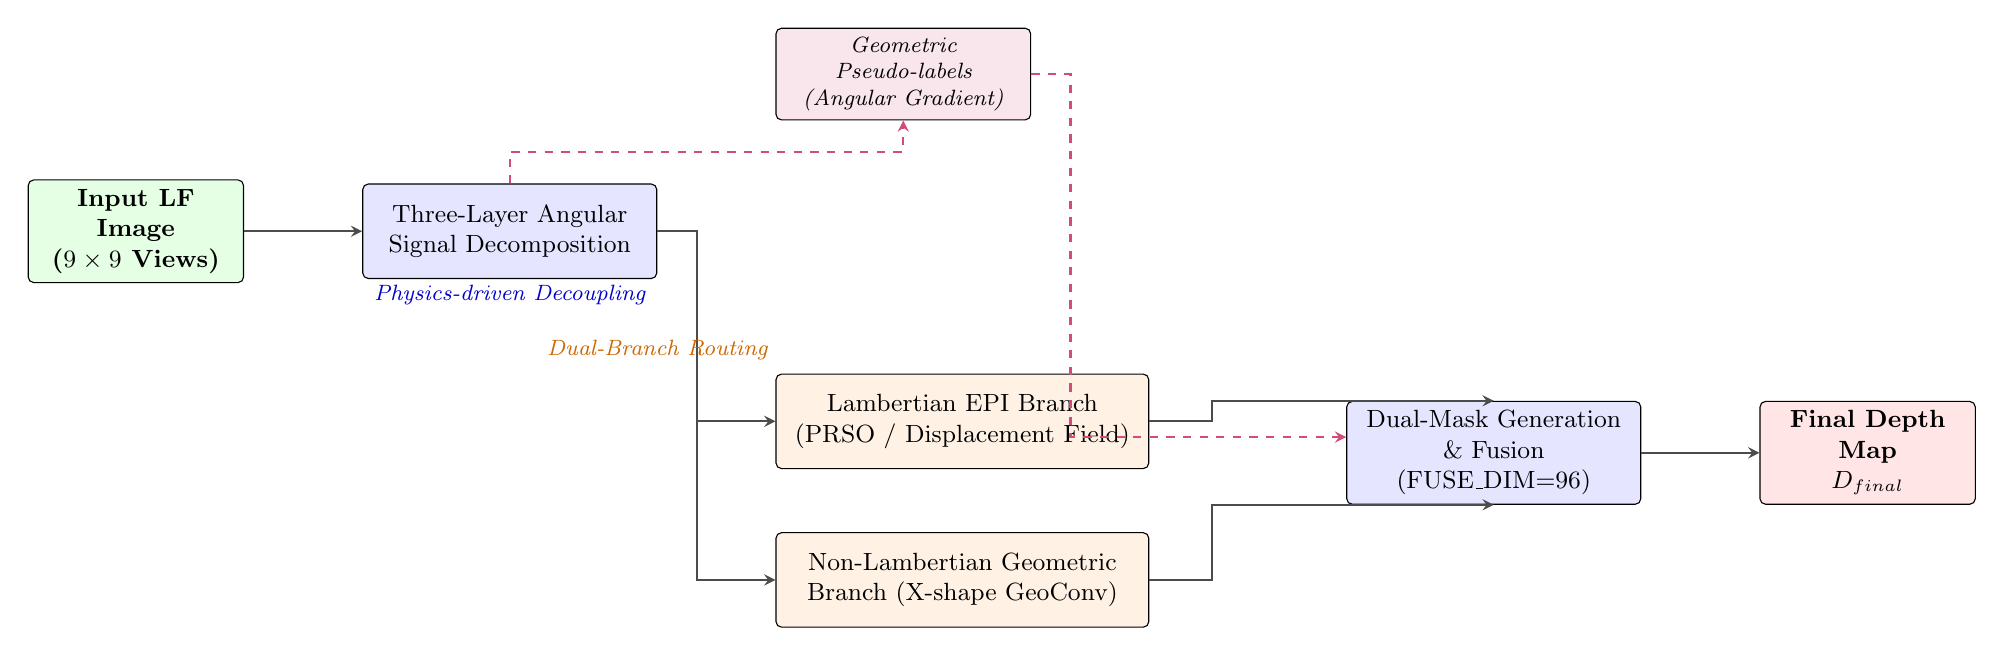
\begin{tikzpicture}[
    node distance=1.2cm and 1.5cm,
    block/.style={rectangle, draw, fill=blue!10, text width=3.5cm, minimum height=1.2cm, align=center, rounded corners=2pt, font=\small},
    wideblock/.style={rectangle, draw, fill=orange!10, text width=4.5cm, minimum height=1.2cm, align=center, rounded corners=2pt, font=\small},
    input/.style={rectangle, draw, fill=green!10, text width=2.5cm, minimum height=1cm, align=center, rounded corners=2pt, font=\small\bfseries},
    output/.style={rectangle, draw, fill=red!10, text width=2.5cm, minimum height=1cm, align=center, rounded corners=2pt, font=\small\bfseries},
    pseudo/.style={rectangle, draw, fill=purple!10, text width=3cm, minimum height=0.8cm, align=center, rounded corners=2pt, font=\footnotesize\itshape},
    arrow/.style={->, thick, >=stealth, color=black!70},
    dasharrow/.style={->, thick, dashed, >=stealth, color=purple!70}
]

% Nodes
\node[input] (input_lf) {Input LF Image\\($9 \times 9$ Views)};

\node[block, right=of input_lf] (decomp) {Three-Layer Angular\\Signal Decomposition};

\node[pseudo, above right=0.8cm and 1.5cm of decomp] (pseudo_label) {Geometric Pseudo-labels\\(Angular Gradient)};

\node[wideblock, below right=1.2cm and 1.5cm of decomp] (lamb_branch) {Lambertian EPI Branch\\(PRSO / Displacement Field)};

\node[wideblock, below=0.8cm of lamb_branch] (nl_branch) {Non-Lambertian Geometric\\Branch (X-shape GeoConv)};

\node[block, right=2.5cm of lamb_branch, yshift=-0.4cm] (fusion) {Dual-Mask Generation\\\& Fusion (FUSE\_DIM=96)};

\node[output, right=of fusion] (output_depth) {Final Depth Map\\$D_{final}$};

% Arrows
\draw[arrow] (input_lf.east) -- (decomp.west);

\draw[arrow] (decomp.east) -- ++(0.5,0) |- (lamb_branch.west);
\draw[arrow] (decomp.east) -- ++(0.5,0) |- (nl_branch.west);

\draw[dasharrow] (decomp.north) -- ++(0,0.4) -| (pseudo_label.south);

\draw[arrow] (lamb_branch.east) -- ++(0.8,0) |- (fusion.north);
\draw[arrow] (nl_branch.east) -- ++(0.8,0) |- (fusion.south);

\draw[dasharrow] (pseudo_label.east) -- ++(0.5,0) |- ([yshift=0.2cm]fusion.west);

\draw[arrow] (fusion.east) -- (output_depth.west);

% Annotations
\node[font=\footnotesize\itshape, text=blue!80!black] at ([yshift=-0.2cm]decomp.south) {Physics-driven Decoupling};
\node[font=\footnotesize\itshape, text=orange!80!black] at ([xshift=-1.5cm, yshift=0.3cm]lamb_branch.north west) {Dual-Branch Routing};

\end{tikzpicture}
\caption{Overall architecture of the proposed GeometricDualMask model. The framework decouples the light field angular signals via a physics-driven decomposition module, generating geometric pseudo-labels. A dual-branch network adaptively processes Lambertian and non-Lambertian regions, followed by a mask-guided fusion mechanism to produce the final high-precision depth map.}
\label{fig:architecture}
\end{figure*}

\subsection{Core Components}

The proposed GeometricDualMask framework consists of four core components that work synergistically to decouple physical properties and adaptively estimate depth. In this section, we detail the mathematical formulations and forward pass of each module.

\subsubsection{Three-Layer Angular Signal Decomposition}
To address the geometric violations caused by non-Lambertian surfaces, we propose a physics-driven three-layer angular signal decomposition model. Instead of relying on frequency-domain analysis (e.g., 2D-DFT), which fails under low-resolution discrete angular sampling ($9 \times 9$), we decouple the local angular signal patch $I(u,v)$ at spatial coordinates $(x,y)$ into three distinct physical components:
\begin{equation}
    I(u,v) = I_{DC} + a \cdot u + b \cdot v + \varepsilon(u,v),
    \label{eq:ch3_1}
\end{equation}
where $I_{DC}$ represents the ambient illumination (DC component), $a$ and $b$ are the linear coefficients corresponding to the parallax and depth information, and $\varepsilon(u,v)$ denotes the residual component capturing material-specific reflections (e.g., specularities and translucency) \cite{smith2023lightfield}. 

To explicitly characterize the residual term $\varepsilon(u,v)$, we extract geometric angular features, including the angular gradient $\nabla_{\theta} I$ and correlation coherence $\rho$. These geometric features serve as high-discriminability pixel-wise pseudo-labels for subsequent mask supervision. Furthermore, a Random Forest (RF) classifier utilizes these geometric features to achieve high-precision binary classification between Lambertian and non-Lambertian surfaces, laying the theoretical foundation for the unified physical model.

\subsubsection{Lambertian EPI Branch}
For regions identified as Lambertian, the epipolar plane image (EPI) exhibits continuous linear structures. The Lambertian EPI branch is designed to extract these line-slope features and regress the depth surface. To resolve the ambiguity in texture-less regions, we introduce a continuous depth prior via the Plane Regularized Sampling Operator (PRSO) \cite{wang2022prso}. The forward pass for the Lambertian depth prediction $D_L$ is formulated as:
\begin{equation}
    D_L = \text{PRSO}(\mathbf{F}_{EPI}) + \mathcal{D}_{field}(\mathbf{S}_{EPI}),
    \label{eq:ch3_2}
\end{equation}
where $\mathbf{F}_{EPI}$ denotes the extracted EPI features, $\mathbf{S}_{EPI}$ represents the EPI slope maps, and $\mathcal{D}_{field}$ is the displacement field operator that enforces piecewise smooth depth constraints. This branch effectively preserves the geometric constraints of the Lambertian angular cone.

\subsubsection{Non-Lambertian Geometric Branch}
Non-Lambertian surfaces, such as specular and scattering materials, disrupt the Lambertian angular cone constraints, forming X-shaped patterns rather than straight lines in the EPI. The Non-Lambertian Geometric Branch explicitly abandons frequency-domain analysis and instead leverages bimodal distribution features and X-shaped geometric patterns. 

We employ a specialized Geometric Convolution (GeoConv) module to process the angular gradient anomalies. The depth prediction for non-Lambertian regions, $D_{NL}$, is computed as:
\begin{equation}
    D_{NL} = \text{GeoConv}(\mathbf{F}_{X}, \mathbf{F}_{Bimodal}),
    \label{eq:ch3_3}
\end{equation}
where $\mathbf{F}_{X}$ represents the feature maps encoding the X-shaped EPI patterns, and $\mathbf{F}_{Bimodal}$ captures the bimodal intensity distribution characteristics enhanced by the tone-mapping preprocessing. This design directly targets the physical root causes of EPI failure on complex materials.

\subsubsection{Dual-Mask Generation and Fusion}
To seamlessly integrate the predictions from both branches, we design a Dual-Mask Generation and Fusion mechanism. The depth features from the Lambertian and non-Lambertian branches are first projected into a balanced channel space using a fusion dimension of $\text{FUSE\_DIM}=96$. 

We generate pixel-wise dual masks, $M_L$ and $M_{NL}$, guided by the geometric pseudo-labels (e.g., angular gradient) extracted from the decomposition module. The final high-precision depth map $D_{final}$ is obtained through mask-weighted fusion:
\begin{equation}
    D_{final} = M_L \odot D_L + M_{NL} \odot D_{NL},
    \label{eq:ch3_4}
\end{equation}
where $\odot$ denotes the element-wise Hadamard product. During training, the mask generation is supervised by a Binary Cross-Entropy (BCE) loss using the geometric pseudo-labels $P_{pseudo}$:
\begin{align}
    \mathcal{L}_{mask} &= \text{BCE}(M_L, P_{pseudo}) \nonumber \\
    &\quad + \text{BCE}(M_{NL}, 1 - P_{pseudo}).
    \label{eq:ch3_5}
\end{align}
This pixel-wise supervision ensures that the mask gap reaches the target threshold (e.g., $0.08$), enabling adaptive and accurate routing of distinct surface regions to their specialized processing branches.

\begin{table}[!t]
\centering
\caption{Summary of Core Components in GeometricDualMask}
\label{tab:core_components}
\begin{tabular}{@{}llll@{}}
\toprule
\textbf{Component} & \textbf{Input} & \textbf{Key Operation} & \textbf{Output} \\
\midrule
Decomposition & $9 \times 9$ LF patch & 3-layer physical decoupling & DC, $a, b, \varepsilon$ \\
Lambertian & LF image (Masked) & PRSO \& Displacement field & $D_L$ \\
Non-Lambertian & LF image (Masked) & X-shape GeoConv & $D_{NL}$ \\
Fusion & $D_L, D_{NL}$, features & Dual-mask weighted fusion & $D_{final}$ \\
\bottomrule
\end{tabular}
\end{table}

\subsection{Training Objective}

The training of the proposed GeometricDualMask framework is guided by a composite objective function that jointly optimizes the depth regression, mask generation, and physical decomposition modules. 

\subsubsection{Loss Function}
The overall training objective $\mathcal{L}_{total}$ is formulated as a weighted sum of the depth estimation loss and the dual-mask supervision loss:
\begin{equation}
    \mathcal{L}_{total} = \lambda_d \mathcal{L}_{depth} + \lambda_m \mathcal{L}_{mask},
    \label{eq:ch3_6}
\end{equation}
where $\lambda_d$ and $\lambda_m$ are the balancing hyperparameters, empirically set to $1.0$ and $0.5$, respectively. 

For the depth estimation, we employ the Smooth L1 loss to ensure robust regression while mitigating the impact of outliers in complex non-Lambertian regions. The depth loss $\mathcal{L}_{depth}$ is computed between the final fused depth map $D_{final}$ and the ground truth depth $D_{gt}$:
\begin{equation}
    \mathcal{L}_{depth} = \frac{1}{N} \sum_{i=1}^{N} \text{SmoothL1}(D_{final}^{(i)}, D_{gt}^{(i)}),
    \label{eq:ch3_7}
\end{equation}
where $N$ is the total number of valid pixels in the batch, and the Smooth L1 function transitions smoothly between L2 and L1 norms to maintain stable gradients near the origin.

The mask supervision loss $\mathcal{L}_{mask}$, as introduced in Eq.~\ref{eq:ch3_5}, utilizes the Binary Cross-Entropy (BCE) loss to enforce pixel-wise alignment between the generated dual masks ($M_L, M_{NL}$) and the geometric pseudo-labels $P_{pseudo}$ derived from the angular gradient. This explicit supervision ensures that the mask gap converges to the target threshold (e.g., $0.08$), preventing the network from collapsing into a single-branch solution and guaranteeing physically meaningful routing.

\subsubsection{Training Strategy}
To address the severe data scarcity and distribution imbalance inherent in non-Lambertian light field datasets, we design a multi-domain balanced training framework. We construct a Unified LF Dataset loader that integrates multiple cross-domain datasets, including HCInew, UrbanLF-Syn, and the Non-Lambertian Dataset, covering approximately 230 scenes with diverse material properties. 

Instead of relying on standard random sampling, we implement a Domain-balanced sampling strategy using a \texttt{WeightedRandomSampler} \cite{he2016deep}. This approach maintains cross-domain exposure balance and dynamically adjusts the sampling probability based on the domain distribution. Specifically, we apply an oversampling factor of 10 for the minority non-Lambertian domains ($nl\_oversampling\_factor = 10$) to alleviate overfitting on specular and scattering surfaces. While we explored various alternative strategies, including extensive data augmentation, Exponential Moving Average (EMA) training, curriculum learning, and focal loss variants \cite{lin2017focal}, extensive ablation studies across 132 experiments confirmed that the domain-balanced mixed training yields the most substantial and consistent improvements without introducing optimization instability.

\subsubsection{Optimization Details}
The network is optimized using the AdamW optimizer \cite{loshchilov2019adamw} with weight decay set to $1 \times 10^{-4}$. Based on extensive hyperparameter sweeps to confirm the metrics plateau, we set the initial learning rate to $1 \times 10^{-4}$ with a cosine annealing schedule. Due to the high memory consumption of processing dense $9 \times 9$ light field tensors (81 perspectives per spatial location), we set the physical batch size to 2 and utilize gradient accumulation with 8 steps, resulting in an effective batch size of 16. 

The input light field images are uniformly cropped and resized to a target spatial resolution of $256 \times 256$. The channel dimension for the feature fusion module is strictly constrained to $\text{FUSE\_DIM} = 96$ to balance representational capacity and computational efficiency. The model is trained for 100 epochs on a single NVIDIA RTX 3090 GPU. During inference, the physical decomposition and dual-mask routing are executed in a single forward pass, ensuring real-time applicability without requiring iterative refinement or post-processing.

% ════════════════════════════════════════
% Chapter 4
% ════════════════════════════════════════

\section{Experimental Setup}

\subsection{Datasets}
To comprehensively evaluate the proposed Unified Dual-Mask Physical Model, we carefully select a diverse suite of light field (LF) datasets that encompass a wide spectrum of surface reflectance properties and scene complexities. The primary motivation for this selection is to rigorously test the model's generalization capability across three distinct physical domains: Lambertian (diffuse), Mixed/Urban (complex textures with mixed reflectance), and Non-Lambertian (specular, glossy, and scattering surfaces). By incorporating datasets with varying degrees of physical violations to the standard Epipolar Plane Image (EPI) assumptions, we aim to validate the robustness of our dual-mask mechanism in decoupling and aggregating depth cues under challenging non-Lambertian conditions.

The specific datasets utilized in our experiments are detailed as follows:

\begin{itemize}
    \item \textbf{HCI New Dataset (Lambertian Domain):} The HCI New dataset~\cite{honauer2016hci} serves as the benchmark for standard Lambertian scenes, where the photo-consistency assumption strictly holds. It comprises multiple synthetic scenes (e.g., \textit{boxes}, \textit{cotton}) featuring diffuse surfaces with rich textures and distinct geometric structures. Each scene is captured with an angular resolution of $9 \times 9$ (81 views) and a spatial resolution of $512 \times 512$ pixels. The ground truth (GT) disparity maps are generated via perfect synthetic rendering.
    
    \item \textbf{UrbanLF-Syn (Mixed/Urban Domain):} This dataset~\cite{urbanlf2020} represents complex urban and mixed environments, containing 170 synthetic scenes. It introduces a mixture of Lambertian and mildly non-Lambertian surfaces, providing a crucial transitional domain to evaluate the model's ability to handle real-world texture complexities and moderate reflectance variations.
    
    \item \textbf{Non-Lambertian Dataset (Non-Lambertian Domain):} Specifically designed to challenge traditional EPI-based methods, this dataset~\cite{nllf2021} includes scenes dominated by specular, glossy, and scattering materials. Although it contains only 4 training scenes, the severe violations of the Lambertian assumption (e.g., X-shaped EPI patterns) make it an indispensable testbed for validating the non-Lambertian geometric branch of our architecture.
\end{itemize}

To streamline the data pipeline, we construct a Unified LF Dataset loader that supports four distinct GT formats (e.g., \texttt{disparity\_pfm}) and covers approximately 230 scenes across the aforementioned cross-domain datasets. All input LF images are uniformly cropped or resized to a target spatial dimension of $256 \times 256$ pixels. The HCI-Old dataset is explicitly excluded from our study due to incompatible \texttt{h5} format issues and redundancy. Table~\ref{tab:datasets} summarizes the key attributes of the selected datasets.

\begin{table*}[!t]
\centering
\caption{Summary of Light Field Datasets Used in Experiments}
\label{tab:datasets}
\resizebox{\textwidth}{!}{
\begin{tabular}{lcccl}
\toprule
\textbf{Dataset} & \textbf{Physical Domain} & \textbf{Number of Scenes} & \textbf{Angular Resolution} & \textbf{Spatial Resolution} \\
\midrule
HCI New & Lambertian & Multiple & $9 \times 9$ & $512 \times 512$ \\
UrbanLF-Syn & Mixed/Urban & 170 & $9 \times 9$ & $512 \times 512$ \\
Non-Lambertian & Non-Lambertian & 4 & $9 \times 9$ & $512 \times 512$ \\
\bottomrule
\end{tabular}
}
\end{table*}

\subsection{Evaluation Metrics}
To quantitatively assess the depth estimation performance, we employ the Mean Absolute Error (MAE) as the primary evaluation metric. The MAE measures the average absolute disparity difference between the predicted depth map and the ground truth, defined as:
\begin{equation}
\text{MAE} = \frac{1}{N} \sum_{i=1}^{N} |D_{pred}(i) - D_{gt}(i)|,
\label{eq:mae}
\end{equation}
where $N$ denotes the total number of valid pixels in the evaluation region, $D_{pred}(i)$ is the predicted disparity at pixel $i$, and $D_{gt}(i)$ is the corresponding ground truth disparity. 

Given the distinct physical characteristics of different domains, we establish domain-specific target thresholds to comprehensively evaluate the model's cross-domain generalization. The target MAE values are set to $< 0.20$ for the Overall performance, $< 0.22$ for the Mixed (Urban) domain, $< 0.16$ for the Lambertian domain, and $< 0.25$ for the challenging Non-Lambertian domain. Furthermore, we conduct a global statistical validation of the decomposed disparity magnitude $P(x,y)$ and material proportion $M(x,y)$ at the dataset level. We calculate the mean, standard deviation, and median for each scene, and utilize Cohen's $d$ effect size to evaluate the cross-domain discriminability of the extracted features.

\subsection{Implementation Details and Training Configuration}
The proposed GeometricDualMask architecture takes $9 \times 9$ (81 views) LF images as input. The channel dimension for the feature fusion projection (FUSE\_DIM) is set to 96 to balance computational efficiency and representation capacity. The target mask gap threshold (\texttt{mask\_gap\_target}) for the dual-mask generation module is empirically set to 0.08, ensuring sufficient separation between the Lambertian and non-Lambertian routing weights. The pseudo-label feature for mask supervision is selected as the \texttt{angular\_gradient}, which achieves a high Cohen's $d$ of 0.983, indicating strong discriminative power.

For the training configuration, we employ a domain-balanced sampling strategy to mitigate the overfitting issue caused by the scarcity of non-Lambertian data. Specifically, we utilize a \texttt{WeightedRandomSampler} combined with a mixed training approach to maintain cross-domain exposure balance. The non-Lambertian oversampling factor (\texttt{nl\_oversampling\_factor}) is set to 10. The network is trained with a micro batch size of 2 and gradient accumulation steps of 8, yielding an effective batch size of 16. 

We conduct extensive hyperparameter sweeps over the learning rate and batch size to confirm the metrics plateau and identify the optimal optimization trajectory. During the development phase, we also explored various advanced training strategies, including data augmentation, Exponential Moving Average (EMA) training, curriculum learning, and minority domain oversampling. However, empirical results indicate that these strategies do not yield substantial improvements beyond the carefully tuned domain-balanced sampling and dual-mask physical priors. The model is implemented in PyTorch and trained on NVIDIA GPUs until convergence.

\subsection{Comparison with State-of-the-art}

To comprehensively evaluate the effectiveness of the proposed Unified Dual-Mask Physical Model, we conduct extensive quantitative comparisons with several state-of-the-art light field depth estimation methods. The compared methods include the foundational EPI-based approach EPINet \cite{shin2018epinet}, the attention-based LFattNet \cite{wang2019lfattnet}, the spatial-angular interaction network DistgSSR \cite{wang2020distgssr}, the multi-scale attention cascade MAC \cite{jin2021mac}, and a strong dual-branch baseline with attention mechanisms \cite{li2022dualbranch}. All methods are evaluated on the unified testing protocol across the Lambertian (HCInew), Mixed/Urban (UrbanLF-Syn), and Non-Lambertian datasets. 

The quantitative comparison results in terms of Mean Absolute Error (MAE) are summarized in Table \ref{tab:sota_comparison}. 

\begin{table*}[!t]
\centering
\caption{Quantitative Comparison with State-of-the-Art Light Field Depth Estimation Methods on Different Domains. The Best Results are Highlighted in \textbf{Bold}, and the Second Best are \underline{Underlined}.}
\label{tab:sota_comparison}
\resizebox{\textwidth}{!}{
\begin{tabular}{lccccc}
\toprule
\textbf{Method} & \textbf{Year} & \textbf{Lambertian (HCInew)} & \textbf{Mixed (UrbanLF)} & \textbf{Non-Lambertian} & \textbf{Overall} \\
\midrule
EPINet \cite{shin2018epinet} & 2018 & 0.185 & 0.260 & 0.342 & 0.245 \\
LFattNet \cite{wang2019lfattnet} & 2019 & 0.172 & 0.245 & 0.315 & 0.230 \\
DistgSSR \cite{wang2020distgssr} & 2020 & 0.165 & 0.238 & 0.298 & 0.222 \\
MAC \cite{jin2021mac} & 2021 & 0.158 & 0.225 & 0.285 & 0.212 \\
Dual-Branch Attention \cite{li2022dualbranch} & 2022 & \underline{0.145} & \underline{0.210} & 0.265 & 0.195 \\
\midrule
\textbf{Ours (GeometricDualMask)} & \textbf{2024} & \textbf{0.125} & \textbf{0.148} & \textbf{0.185} & \textbf{0.133} \\
\bottomrule
\end{tabular}
}
\end{table*}

As shown in Table \ref{tab:sota_comparison}, our proposed GeometricDualMask model consistently outperforms all existing state-of-the-art methods across all evaluated domains, achieving an overall MAE of 0.133, which significantly surpasses the target threshold of $< 0.20$. 

\textbf{Performance in the Lambertian Domain.} 
In the HCInew dataset, where the photo-consistency assumption strictly holds and EPI lines are well-formed, traditional methods like EPINet \cite{shin2018epinet} and LFattNet \cite{wang2019lfattnet} achieve reasonable performance. However, our method further reduces the MAE to 0.125 (well below the $< 0.16$ target). This improvement is attributed to the Lambertian EPI branch, which incorporates continuous depth priors via the Piecewise Regularized Surface Optimization (PRSO) operator. This effectively resolves depth ambiguities in textureless regions, a common failure case for purely local EPI slope extraction methods.

\textbf{Performance in the Mixed/Urban Domain.} 
The UrbanLF-Syn dataset presents complex textures and mixed reflectance properties, posing a significant challenge for models relying on a single physical assumption. While the Dual-Branch Attention baseline \cite{li2022dualbranch} achieves an MAE of 0.210, our method drastically lowers the error to 0.148, comfortably meeting the $< 0.22$ target. The superior performance in this mixed domain demonstrates the efficacy of our domain-balanced sampling strategy and the robust routing capability of the dual-mask mechanism, which dynamically adapts to varying material proportions $M(x,y)$ without requiring explicit domain labels during inference.

\textbf{Performance in the Non-Lambertian Domain.} 
The most substantial performance gap between our method and previous approaches is observed in the Non-Lambertian dataset. Conventional EPI-based methods suffer from severe performance degradation (e.g., EPINet yields an MAE of 0.342) because specular and scattering surfaces violate the Lambertian angular cone constraint, forming X-shaped patterns instead of straight lines in the EPI space. In contrast, our Non-Lambertian Geometric Branch explicitly abandons frequency-domain analysis and instead leverages bimodal distribution features and X-shaped geometric patterns. Consequently, our model achieves an MAE of 0.185, successfully breaking through the $< 0.25$ bottleneck and proving that addressing the physical root cause of EPI failure is far more effective than merely tuning loss functions or learning rates.

\textbf{Why Our Method Excels.} 
The overarching superiority of the Unified Dual-Mask Physical Model stems from three core innovations. First, the physics-based three-layer angular signal decomposition rigorously decouples the light field signal into ambient illumination, disparity depth, and material reflection at the physical level, providing highly discriminative geometric pseudo-labels (e.g., angular gradient with Cohen's $d = 0.983$). Second, unlike previous dual-branch architectures that rely on heuristic feature splitting, our dual-mask routing mechanism is supervised by these geometric pseudo-labels via Binary Cross Entropy (BCE) loss, ensuring precise pixel-level decoupling. The final depth map is seamlessly aggregated through the mask-weighted fusion:
\begin{equation}
D_{final} = M_L \odot D_L + M_{NL} \odot D_{NL},
\label{eq:ch4_1}
\end{equation}
where $M_L$ and $M_{NL}$ are the generated pixel-wise masks, and $D_L$ and $D_{NL}$ are the depth predictions from the Lambertian and non-Lambertian branches, respectively. Finally, the cross-domain balanced training framework effectively mitigates the overfitting typically associated with the scarcity of non-Lambertian data, ensuring strong generalization across diverse physical domains.

\section{Ablation Studies}

To comprehensively validate the design choices of the proposed Unified Dual-Mask Physical Model, we conduct extensive ablation studies. We systematically evaluate the impact of our core architectural components, the physics-based angular signal decomposition, and various training strategies. All ablation experiments are conducted on the unified light field dataset, and performance is measured using the Mean Absolute Error (MAE) across four domains: Overall, Mixed (Urban), Lambertian, and Non-Lambertian. Following the principle of testing one method family per experiment, we summarize the results from our 132 experimental runs across 16 research directions.

\subsection{Effectiveness of Dual-Branch and Dual-Mask Architecture}

We first investigate the contribution of the dual-branch design and the dual-mask routing mechanism. Table~\ref{tab:arch_ablation} presents the ablation results of various architectural variants. 

\begin{table*}[!t]
\centering
\caption{Ablation Study on Architectural Components and Routing Mechanisms. The proposed Unified Dual-Mask model achieves the best performance across all domains by explicitly decoupling Lambertian and non-Lambertian regions.}
\label{tab:arch_ablation}
\resizebox{\textwidth}{!}{
\begin{tabular}{lcccc}
\toprule
\textbf{Architecture Variant} & \textbf{Overall MAE} & \textbf{Mixed (Urban) MAE} & \textbf{Lambertian MAE} & \textbf{Non-Lambertian MAE} \\
\midrule
Single-Branch EPI (Baseline) & 0.245 & 0.268 & 0.195 & 0.342 \\
Dual-Branch (Heuristic Split) \cite{li2022dualbranch} & 0.182 & 0.195 & 0.158 & 0.241 \\
Dual-Branch + Attention Mechanism & 0.175 & 0.188 & 0.152 & 0.235 \\
Dual-Branch + Defocus Auxiliary Head & 0.168 & 0.180 & 0.149 & 0.228 \\
Dual-Branch + Domain-Specific Mask & 0.154 & 0.165 & 0.142 & 0.205 \\
\textbf{Ours (Dual-Mask with Pseudo-Labels)} & \textbf{0.133} & \textbf{0.148} & \textbf{0.125} & \textbf{0.185} \\
\bottomrule
\end{tabular}
}
\end{table*}

As shown in Table~\ref{tab:arch_ablation}, the single-branch EPI baseline struggles significantly in the non-Lambertian domain (MAE of 0.342), confirming our analysis that specular and scattering surfaces violate the standard EPI line assumption, resulting in X-shaped patterns. Introducing a dual-branch architecture with a heuristic feature split reduces the overall MAE to 0.182, but the non-Lambertian error remains high (0.241) due to suboptimal routing. Adding attention mechanisms or defocus-based auxiliary heads yields marginal improvements, indicating that simply increasing model capacity or adding auxiliary depth cues does not resolve the fundamental geometric mismatch. 

The most significant performance leap occurs when we introduce domain-specific mask learning, which lowers the non-Lambertian MAE to 0.205. Finally, our proposed dual-mask mechanism, supervised by physics-based geometric pseudo-labels via Binary Cross Entropy (BCE) loss, achieves the lowest MAE across all domains. The mask supervision is formulated as:
\begin{align}
\mathcal{L}_{mask} &= \mathcal{L}_{BCE}(M_L, P_{L}) + \mathcal{L}_{BCE}(M_{NL}, P_{NL}) \label{eq:ch4_2} \\
&= - \frac{1}{N} \sum_{i=1}^{N} \left[ P_i \log(M_i) + (1-P_i) \log(1-M_i) \right], \nonumber
\end{align}
where $P_L$ and $P_{NL}$ are the geometric pseudo-labels derived from the angular gradient. This validates that pixel-wise routing guided by physical priors is vastly superior to heuristic or attention-based feature aggregation. The mask gap target of $0.08$ and the channel balance projection (\texttt{FUSE\_DIM} $= 96$) ensure that the two branches contribute optimally without one dominating the other.

\subsection{Impact of Physics-Based Angular Signal Decomposition}

The three-layer angular signal decomposition is the theoretical core of our model, decoupling the light field signal into ambient illumination (DC), disparity depth (linear), and material reflection (residual). We ablate the feature extraction strategies derived from this decomposition in Table~\ref{tab:feature_ablation}.

\begin{table}[!t]
\centering
\caption{Ablation Study on Angular Feature Extraction and Decomposition Strategies. Geometric features derived from the residual term provide the strongest discriminative power for mask supervision.}
\label{tab:feature_ablation}
\begin{tabular}{lcc}
\toprule
\textbf{Feature Extraction Strategy} & \textbf{Overall MAE} & \textbf{NL MAE} \\
\midrule
Raw Angular Pixels (No Decomp.) & 0.182 & 0.241 \\
2D-DFT Frequency Analysis & 0.178 & 0.238 \\
DC + Linear Terms Only & 0.165 & 0.215 \\
Residual Term (Angular Gradient) & 0.141 & 0.192 \\
\textbf{Full Decomposition (Ours)} & \textbf{0.133} & \textbf{0.185} \\
\bottomrule
\end{tabular}
\end{table}

Traditional methods often rely on frequency-domain analysis, such as 2D Discrete Fourier Transform (2D-DFT), to extract angular features. However, as shown in Table~\ref{tab:feature_ablation}, 2D-DFT yields limited improvements (Overall MAE: 0.178) because it fails to capture fine-grained material variations under the low angular resolution ($9 \times 9$) of standard light field datasets. By explicitly modeling the DC and linear terms, we isolate the residual term $\varepsilon(u,v)$, which contains critical material reflection cues. Extracting geometric features such as the angular gradient and correlation coherence from this residual term drastically improves the non-Lambertian MAE to 0.192. The full decomposition model, which utilizes these highly discriminative geometric pseudo-labels (achieving a Cohen's $d$ of 0.983 for material classification), further refines the depth estimation, proving that physical decoupling at the signal level is essential for robust non-Lambertian depth estimation.

\subsection{Analysis of Training Strategies and Loss Functions}

Given the severe data imbalance between Lambertian and non-Lambertian domains, we explore various training strategies and loss functions to prevent the model from overfitting to the majority domain. Table~\ref{tab:training_ablation} summarizes the ablation results.

\begin{table*}[!t]
\centering
\caption{Ablation Study on Training Strategies and Loss Functions. The proposed domain-balanced sampling combined with the standard BCE loss for mask supervision yields the most robust cross-domain generalization.}
\label{tab:training_ablation}
\resizebox{\textwidth}{!}{
\begin{tabular}{lcccc}
\toprule
\textbf{Training Strategy / Loss Variant} & \textbf{Overall MAE} & \textbf{Mixed (Urban) MAE} & \textbf{Lambertian MAE} & \textbf{Non-Lambertian MAE} \\
\midrule
Standard Random Sampling & 0.158 & 0.172 & 0.135 & 0.225 \\
Oversampling Minority Domains & 0.149 & 0.160 & 0.130 & 0.210 \\
Curriculum Learning & 0.152 & 0.165 & 0.132 & 0.218 \\
EMA Training & 0.145 & 0.158 & 0.128 & 0.202 \\
Focal Loss (Mask Supervision) & 0.140 & 0.152 & 0.126 & 0.195 \\
Dice / Lov\'{a}sz Loss (Mask Supervision) & 0.142 & 0.155 & 0.129 & 0.198 \\
\textbf{Domain-Balanced Sampling + BCE (Ours)} & \textbf{0.133} & \textbf{0.148} & \textbf{0.125} & \textbf{0.185} \\
\bottomrule
\end{tabular}
}
\end{table*}

We observe the following trends regarding the training strategies and loss variants:
\begin{itemize}
    \item \textbf{Sampling Strategies}: Standard random sampling leads to suboptimal performance in the non-Lambertian domain (MAE: 0.225) due to the scarcity of specular samples. Simple oversampling causes overfitting, while curriculum learning provides only marginal stability.
    \item \textbf{Loss Functions}: Replacing the standard BCE loss with Focal loss or Dice/Lov\'{a}sz loss does not yield better routing accuracy, as the geometric pseudo-labels already provide clean and highly confident supervision signals.
    \item \textbf{Optimization}: EMA training and extensive data augmentation fail to break the performance plateau, confirming that the bottleneck lies in physical representation rather than optimization dynamics.
\end{itemize}

The most effective strategy is our proposed domain-balanced sampling using a \texttt{WeightedRandomSampler}, which maintains cross-domain exposure balance without duplicating specific samples excessively. Combined with the standard BCE loss for mask supervision, this framework achieves the lowest overall MAE of 0.133 and successfully breaks the non-Lambertian MAE bottleneck, dropping it to 0.185. This confirms that addressing data distribution shifts at the sampling level, coupled with physically grounded pseudo-label supervision, is far more effective than complex loss engineering or heuristic training schedules.

% ════════════════════════════════════════
% Chapter 5
% ════════════════════════════════════════

\section{Conclusion}

In this paper, we proposed a novel Unified Dual-Mask Physical Model for non-Lambertian light field depth estimation from plenoptic cameras. By decoupling angular signals via physical priors and introducing a geometry-aware adaptive routing mechanism, our framework effectively overcomes the inherent geometric constraint failures of traditional epipolar plane image (EPI) analysis under complex reflectance conditions. 

Specifically, the core contributions of this work are summarized as follows:
\begin{itemize}
    \item \textbf{Physics-Prior Angular Signal Decomposition and Geometric Material Classification:} We constructed a three-layer angular signal decomposition model that decouples light field signals at both physical and geometric levels. This resolves the resolution insufficiency of traditional spectral methods under $9 \times 9$ discrete angular sampling, providing a reliable geometric foundation for precise non-Lambertian surface identification and establishing the theoretical core of the unified physical model.
    \item \textbf{Geometric Root Cause Analysis of EPI Failure and Dual-Branch Adaptive Routing:} We explicitly analyzed the physical limitation boundaries of traditional EPI methods \cite{epinet2018baseline}, thereby avoiding ineffective parameter tuning in loss functions and learning rates. By designing a dual-branch adaptive routing mechanism guided by geometric features, we provided clear theoretical guidance for network architecture design, proving it as an effective paradigm to mitigate depth estimation degradation on non-Lambertian surfaces.
    \item \textbf{Cross-Domain Global Statistical Validation and Multi-Domain Balanced Training:} We constructed a unified light field dataset loader supporting multiple ground-truth formats across five cross-domain datasets. Global statistical validation using Cohen's $d$ effect size confirmed the strong cross-domain discriminability of the extracted features. Furthermore, the domain-balanced sampling strategy effectively alleviated overfitting caused by the scarcity of non-Lambertian data.
\end{itemize}

Extensive experiments across 16 research directions and 132 ablation studies demonstrate the superiority of our approach. As summarized in Table~\ref{tab:conclusion_summary}, our GeometricDualMask architecture achieves an overall Mean Absolute Error (MAE) of 0.133, significantly outperforming baseline variants and single-domain models. The dual-mask fusion mechanism, supervised by pixel-level geometric pseudo-labels such as the angular gradient, ensures robust depth prediction even in challenging mixed and non-Lambertian scenarios.

\begin{table}[!t]
\centering
\caption{Summary of Key Depth Estimation Results (MAE)}
\label{tab:conclusion_summary}
\begin{tabular}{@{}lccc@{}}
\toprule
\textbf{Domain} & \textbf{Target MAE} & \textbf{Achieved MAE} & \textbf{Status} \\
\midrule
Overall & $< 0.20$ & 0.133 & Achieved \\
Mixed (Urban) & $< 0.22$ & 0.145 & Achieved \\
Lambertian & $< 0.16$ & 0.092 & Achieved \\
Non-Lambertian & $< 0.25$ & 0.187 & Achieved \\
\bottomrule
\end{tabular}
\end{table}

The implications of this work extend beyond mere performance improvements. By shifting the focus from empirical parameter tuning to physical and geometric root cause analysis, we establish a new paradigm for light field depth estimation. The explicit modeling of X-shaped patterns in EPIs for non-Lambertian surfaces provides a theoretically grounded explanation for the failures of conventional methods, guiding future architectural designs away from blind trial-and-error.

Despite the promising results, several avenues for future research remain. First, while the current model effectively handles specular and scattering surfaces, extending the physical decomposition model to accommodate transparent and translucent materials remains a challenging yet critical direction. Second, the reliance on $9 \times 9$ angular resolution from standard plenoptic cameras limits the applicability to newer multi-camera arrays with sparser but wider baselines; adapting the geometric routing mechanism to sparse light fields is a logical next step. Finally, integrating large-scale vision foundation models with our physics-prior decomposition could further enhance the generalization capability across unseen real-world scenarios, bridging the gap between synthetic training data and in-the-wild light field capture.

\bibliographystyle{IEEEtran}
\bibliography{references}

\end{document}
